\documentclass[a4paper,12pt]{article}
\usepackage[utf8]{inputenc} % Ensure the file is saved with UTF-8 encoding
\usepackage[T1]{fontenc}
\usepackage[spanish]{babel}  % Para escribir en español
\usepackage[a4paper, margin=1in]{geometry}
\usepackage{graphicx}  % Para insertar imágenes
\usepackage{geometry}  % Para ajustar los márgenes
\usepackage{titling}   % Para personalizar el título
\usepackage{setspace}  % Para ajustar el espaciado
\usepackage{fancyhdr}
\usepackage{xcolor}    % Para cambiar el color de la línea del encabezado
\usepackage{listings}
\usepackage{soul}
\usepackage{caption}
\usepackage{wrapfig}
\usepackage{longtable}  % Para dividir en varias páginas
\usepackage{float}  % Ayuda con los entornos flotantes
\usepackage[absolute,overlay]{textpos}
\usepackage[hidelinks]{hyperref}

\geometry{top=2cm,bottom=2cm,left=2cm,right=2cm}  % Márgenes personalizados

\definecolor{mybeige}{RGB}{245, 245, 200}
\definecolor{lightblue}{RGB}{173, 216, 230}
\definecolor{lightgray}{RGB}{240, 240, 240}

% Configuración del encabezado
\pagestyle{fancy}
\fancyhf{}
\fancyhead[L]{
\includegraphics[height=1.5cm]{Imagenes/logounex.png}}  % Imagen a la izquierda
\fancyhead[C]{\raisebox{0.3cm}{\shortstack{Programación en Bases de Datos \\ Proyecto Hacking Ético: SQL Injection}}}  % Texto en el centro
\fancyhead[R]{
\includegraphics[height=1.5cm]{Imagenes/logopoli.png}}  % Imagen a la derecha
\renewcommand{\headrulewidth}{0.4pt}  % Línea debajo del encabezado
\setlength{\headheight}{1.5cm}
\setlength{\headsep}{1cm}
\setlength{\TPHorizModule}{1cm}
\setlength{\TPVertModule}{1cm}

% Configuración del pie de página
\fancyfoot[L]{\textit{Universidad de Extremadura}}  % Texto a la izquierda
\fancyfoot[C]{\thepage}  % Número de página en el centro
\fancyfoot[R]{\textit{Curso 2024-2025}}  % Texto a la derecha
\renewcommand{\footrulewidth}{0.4pt}  % Línea encima del pie de página
\setlength{\footskip}{0cm}

% Configuración del entorno listings para resaltar el código Python
\lstset{
    inputencoding=utf8,
    language=Python,
    basicstyle=\ttfamily\small,
    backgroundcolor=\color{mybeige},
    keywordstyle=\color{blue},
    commentstyle=\color{green},
    stringstyle=\color{red},
    frame=single,
    rulecolor=\color{black},
    showstringspaces=false,
    numbers=left,
    numberstyle=\tiny,
    numbersep=5pt,
    tabsize=4,
    breaklines=true,
    breakatwhitespace=false,
    escapeinside={(*@}{@*)},
    literate={ñ}{{\~n}}1
             {á}{{\'a}}1
             {é}{{\'e}}1
             {í}{{\'i}}1
             {ó}{{\'o}}1
             {ú}{{\'u}}1
             {Á}{{\'A}}1
             {É}{{\'E}}1
             {Í}{{\'I}}1
             {Ó}{{\'O}}1
             {Ú}{{\'U}}1
             {Ñ}{{\~N}}1
}

\lstset{
    language=SQL, % Utiliza SQL como base
    basicstyle=\ttfamily\small,
    backgroundcolor=\color{mybeige},
    keywordstyle=\color{blue}\bfseries,
    commentstyle=\color{green!50!black},
    stringstyle=\color{red},
    frame=single,
    rulecolor=\color{black},
    showstringspaces=false,
    numbers=left,
    numberstyle=\tiny,
    numbersep=5pt,
    tabsize=4,
    breaklines=true,
    breakatwhitespace=false,
    escapeinside={(*@}{@*)},
    morekeywords={
        PROCEDURE, FUNCTION, BEGIN, END, DECLARE, IF, THEN, ELSE, ELSIF, 
        LOOP, FOR, WHILE, EXIT, NULL, EXCEPTION, RAISE, COMMIT, ROLLBACK,
        CURSOR, OPEN, FETCH, CLOSE, GRANT, REVOKE, PACKAGE, TYPE, 
        ALTER, DROP, TRUNCATE, MERGE, USING, VALUES, INTO, SELECT, 
        INSERT, UPDATE, DELETE, RETURN, OUT, IN, INOUT, CONSTANT
    },
    morecomment=[l]{--}, % Comentarios de una línea con --
    morecomment=[s]{/*}{*/}, % Comentarios de bloque
    morestring=[b]', % Cadenas entre comillas simples
    inputencoding=utf8,
    literate={ñ}{{\~n}}1
             {á}{{\'a}}1
             {é}{{\'e}}1
             {í}{{\'i}}1
             {ó}{{\'o}}1
             {ú}{{\'u}}1
             {Á}{{\'A}}1
             {É}{{\'E}}1
             {Í}{{\'I}}1
             {Ó}{{\'O}}1
             {Ú}{{\'U}}1
             {Ñ}{{\~N}}1
}

\lstdefinestyle{console}{
    backgroundcolor=\color{lightgray}, % Color de fondo
    basicstyle=\ttfamily\small,        % Fuente monoespaciada y tamaño pequeño
    breaklines=true,                   % Permitir saltos de línea
    stringstyle=\color{black},
    frame=single,                      % Marco alrededor del código
    framerule=0.5pt,                   % Grosor del marco
    rulecolor=\color{black},           % Color del marco
    xleftmargin=0.5cm,                 % Margen izquierdo
    xrightmargin=0.5cm,                % Margen derecho
    aboveskip=1em,                     % Espacio antes del bloque
    belowskip=1em,                     % Espacio después del bloque
    escapeinside={(*@}{@*)},
    inputencoding=utf8,      % Configura el encoding
    literate={ñ}{{\~n}}1
             {á}{{\'a}}1
             {é}{{\'e}}1
             {í}{{\'i}}1
             {ó}{{\'o}}1
             {ú}{{\'u}}1
             {Á}{{\'A}}1
             {É}{{\'E}}1
             {Í}{{\'I}}1
             {Ó}{{\'O}}1
             {Ú}{{\'U}}1
             {Ñ}{{\~N}}1
}

\begin{document}

\begin{titlepage}
    \centering

    % Imagen de la portada (fotoportada)
    
\includegraphics[width=0.75\textwidth]{Imagenes/fotoportada.png} % Asegúrate de que el archivo esté en la misma carpeta

    \vspace{1cm}

    % Título
    {\Huge \textbf{Programación en Bases de Datos} \par}

    \vspace{0.3cm}

    % Línea de separación
    \rule{\linewidth}{0.1mm}

    \vspace{0.3cm}

    % Subtítulo
    {\LARGE \textbf{Proyecto Hacking Ético: SQL Injection} \par}

    \vspace{1.5cm}

    % Logo de la universidad (logounex)
    
\includegraphics[width=0.25\textwidth]{Imagenes/logounex.png} % Asegúrate de que el archivo esté en la misma carpeta

    \vfill

    % Autor
    {\footnotesize Alejandro Bofill Gonzalez - David Gordillo Burrero - Aarón Manzano Mateos - Ángel Macías Barro \par}

\end{titlepage}

\newpage

\begin{center}
    \renewcommand{\contentsname}{Índice de contenidos}\tableofcontents
\end{center}

\newpage

%Introduccion
\section{Introducción al proyecto}
El presente documento aborda el tema del hacking ético y su aplicación en el estudio de vulnerabilidades en bases 
de datos, con un enfoque particular en las inyecciones SQL. Estas vulnerabilidades constituyen uno de los riesgos 
más comunes y críticos en aplicaciones web que interactúan con bases de datos, permitiendo a los atacantes manipular 
o acceder a información de manera no autorizada. Este trabajo tiene como propósito profundizar en la comprensión de las 
inyecciones SQL, analizando sus tipos, los riesgos asociados y los motivos por los cuales ocurren, para fomentar una perspectiva 
integral de la seguridad en el desarrollo de software.
\vspace{0,5cm}
Para facilitar el aprendizaje práctico y la evaluación de estas vulnerabilidades, se ha desarrollado un laboratorio interactivo 
basado en tecnologías como Flask y Python. Este entorno de simulación permite experimentar con diferentes tipos de inyecciones SQL,
 ofreciendo a los usuarios una experiencia inmersiva y controlada. El laboratorio incluye aplicaciones web diseñadas específicamente
  para emular escenarios reales de inyecciones SQL, permitiendo realizar pruebas tanto en bases de datos Oracle como en PostgreSQL.
   Estas bases de datos, seleccionadas por su relevancia y amplio uso en entornos empresariales, proporcionan un contexto diverso y
    representativo para explorar las técnicas de ataque y sus consecuencias.
    \vspace{0,5cm}

Cada tipo de inyección SQL implementada en el laboratorio ha sido cuidadosamente seleccionada para cubrir un amplio espectro de 
vulnerabilidades. Entre ellas, se encuentran las inyecciones basadas en errores, que explotan los mensajes de error generados por
 la base de datos para extraer información sensible; las inyecciones de tipo "Union Attack", que utilizan la cláusula UNION para 
 combinar resultados de consultas y obtener datos confidenciales; las inyecciones basadas en booleanos, que permiten inferir 
 información mediante la manipulación de condiciones lógicas; y las inyecciones ciegas, que aprovechan diferencias en el 
 comportamiento de la aplicación para deducir detalles de la base de datos sin generar mensajes de error explícitos.
 \vspace{0,5cm}

El diseño del laboratorio incluye páginas individuales para cada tipo de inyección, con formularios de inicio de sesión 
vulnerables, credenciales específicas para realizar las pruebas y explicaciones detalladas sobre el ataque correspondiente.
 Esto permite que los usuarios comprendan tanto la teoría subyacente como la ejecución práctica de cada tipo de inyección. 
 Además, el laboratorio cuenta con documentación complementaria que explica cómo se implementaron las vulnerabilidades y su 
 relevancia en entornos reales, proporcionando una base sólida para que los participantes puedan identificar y mitigar estos 
 riesgos en sus propios proyectos.

 \vspace{0,5cm}
Este trabajo no solo subraya los riesgos asociados con las inyecciones SQL, como el acceso no autorizado a datos confidenciales,
 la alteración o eliminación de información crítica y el compromiso total del servidor de base de datos, sino que también explora 
 las causas más comunes detrás de estas vulnerabilidades. Entre ellas, se encuentran la falta de sanitización de las entradas del
  usuario, el uso de consultas dinámicas inseguras y la ausencia de auditorías de seguridad durante el desarrollo de software. Al
   comprender estos factores, se busca fomentar la adopción de mejores prácticas en la construcción de aplicaciones seguras y
    resilientes.
    
    \vspace{0,5cm}
En conclusión, este proyecto combina un enfoque teórico y práctico para abordar una de las amenazas más relevantes 
en el ámbito de la seguridad informática. Al proporcionar un entorno interactivo y educativo, se espera que este laboratorio 
no solo aumente la conciencia sobre la importancia de prevenir las inyecciones SQL, sino que también capacite a los participantes
 en la identificación, explotación controlada y mitigación de estas vulnerabilidades. Este esfuerzo refleja el compromiso con la 
 promoción de un desarrollo de software más seguro, alineado con los principios del hacking ético y la ciberseguridad.

 \section{Inyección SQL}

    \subsection{¿Qué es una inyección SQL?}

 Imagina que estás en un restaurante y entregas tu orden al mesero. Si todo funciona como debería, el mesero simplemente transmite tu pedido al chef, quien prepara la comida según lo solicitado. Ahora bien, ¿qué pasaría si, en lugar de un pedido normal, decides escribir en la nota algo como: "Quiero una pizza, y además dame acceso a la caja registradora"? Si el sistema del restaurante no tiene medidas para validar las órdenes, es posible que el mensaje llegue al chef, quien podría malinterpretarlo como una instrucción válida y permitirte hacer algo que no deberías poder hacer. Algo similar ocurre con una inyección SQL, pero en el contexto de aplicaciones web y bases de datos.
 \vspace{0,5cm}

 Una inyección SQL es un tipo de ataque en el que un atacante manipula las consultas que una aplicación web hace a su base de datos para ejecutar comandos maliciosos. Esto sucede cuando el sistema no valida adecuadamente las entradas proporcionadas por los usuarios y las trata directamente como parte de la consulta SQL. Por ejemplo, en una página de inicio de sesión, si un usuario malintencionado introduce un texto diseñado específicamente para alterar la lógica de la consulta SQL que valida las credenciales, podría obtener acceso no autorizado al sistema sin necesidad de conocer la contraseña.
 \vspace{0,5cm}

 \begin{figure}[H]
    \centering
    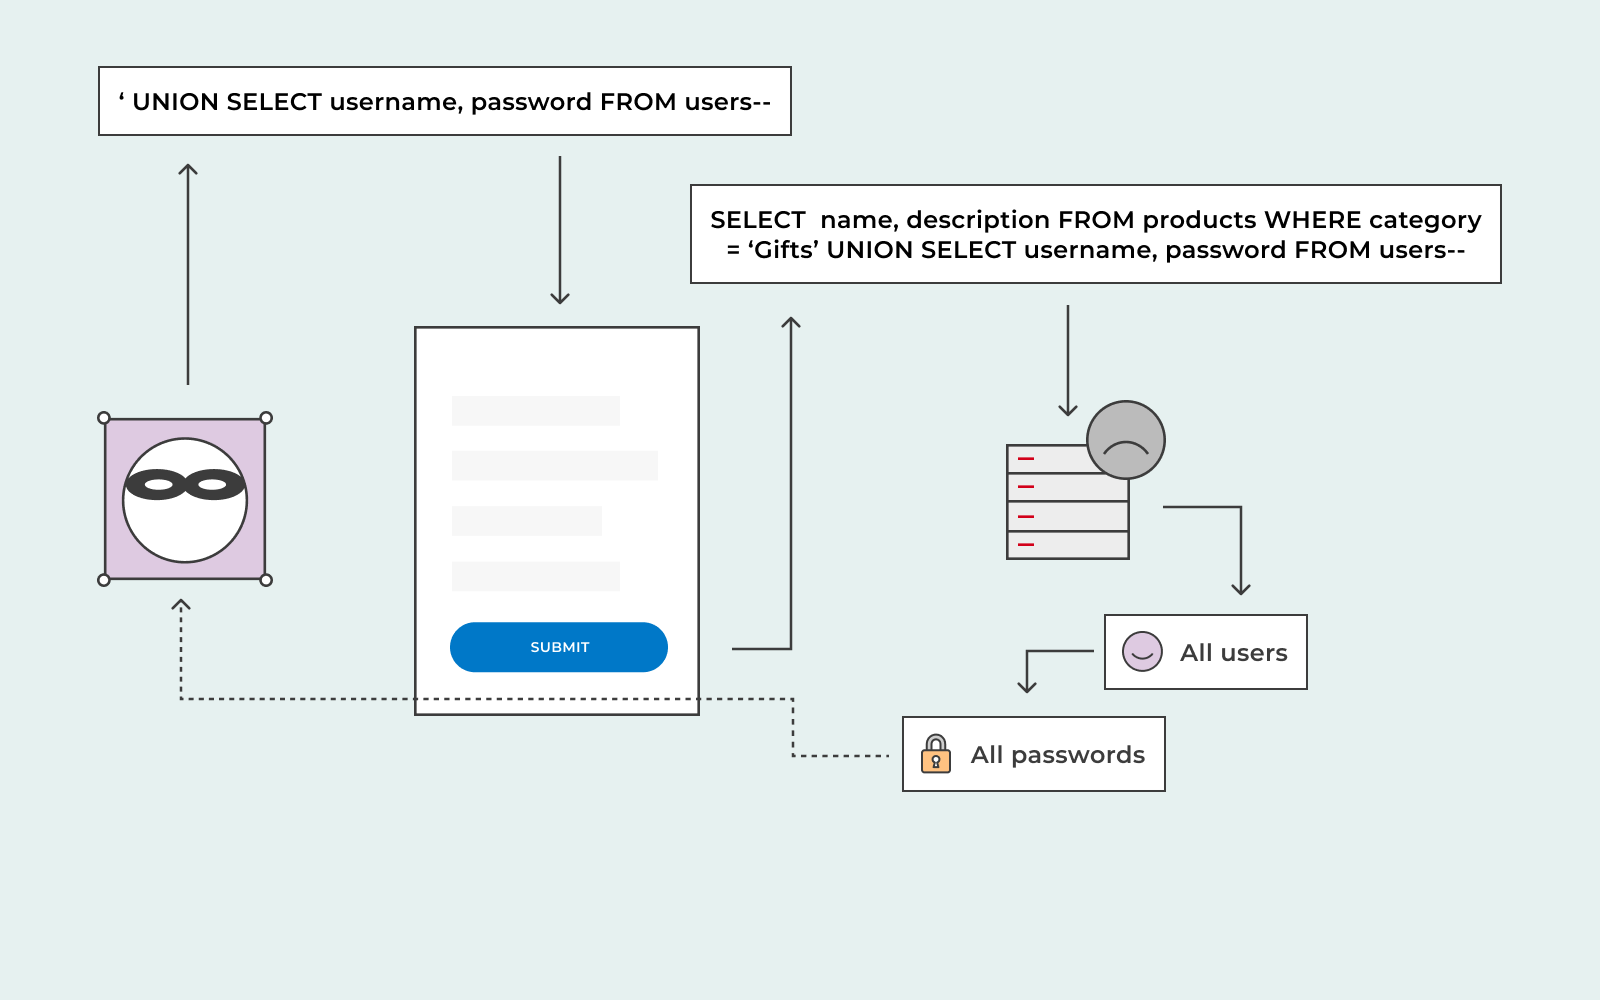
\includegraphics[width=0.8\textwidth]{Imagenes/ejemploSQL.png}
    \caption{Ilustración del flujo de una SQLI}
\end{figure}

\vspace{0,5cm}


 Un caso real que ilustra el impacto de las inyecciones SQL ocurrió en el año 2012, cuando un grupo de atacantes explotó esta vulnerabilidad en una aplicación de LinkedIn. Mediante una inyección SQL, los atacantes lograron acceder a información confidencial de usuarios, incluidos datos de inicio de sesión. Este incidente no solo expuso la información personal de millones de personas, sino que también dañó la reputación de la compañía y resaltó la gravedad de no implementar medidas de seguridad adecuadas.
 \vspace{0,5cm}

 Por ejemplo, imagina una consulta SQL en una aplicación web que maneja la autenticación de usuarios. Una consulta típica podría ser:
 \vspace{0,2cm}

 \begin{lstlisting}[language=SQL]
SELECT * FROM usuarios 
WHERE nombre_usuario = 'usuario' 
AND contraseña = 'contraseña';
 \end{lstlisting}
 \vspace{0,2cm}

 Si el sistema permite que un atacante ingrese algo como \texttt{usuario' OR '1'='1} en lugar del nombre de usuario, la consulta resultante sería:
 \vspace{0,2cm}

 \begin{lstlisting}[language=SQL]
SELECT * FROM usuarios 
WHERE nombre_usuario = 'usuario' OR '1'='1' 
AND contraseña = 'contraseña';
\end{lstlisting}
\vspace{0,2cm}

 La condición \texttt{'1'='1'} siempre es verdadera, lo que significa que el atacante podría acceder al sistema sin necesidad de proporcionar credenciales válidas. Este ejemplo muestra cómo una entrada maliciosa puede alterar la lógica de una consulta SQL, dándole al atacante el control.
 \vspace{0,5cm}

 Las inyecciones SQL pueden tener consecuencias graves, que incluyen el robo de datos confidenciales, la modificación o eliminación de registros, y en casos extremos, el control total del servidor de la base de datos. Además, son una de las vulnerabilidades más comunes en aplicaciones web, según el \textit{OWASP} (Open Web Application Security Project). Sin embargo, prevenirlas no es complicado si se aplican prácticas adecuadas, como el uso de consultas preparadas, la validación estricta de entradas y la implementación de controles de acceso robustos.
 \vspace{0,5cm}

 En resumen, una inyección SQL no es solo un fallo técnico, sino un ejemplo de cómo pequeñas omisiones en la seguridad pueden tener grandes repercusiones. Conocer cómo ocurren y cómo prevenirlas es esencial para cualquier profesional que desarrolle aplicaciones conectadas a bases de datos, ya que no solo se trata de proteger sistemas, sino también la confianza y la información de los usuarios.
 
 \subsection{Causa principal de las inyecciones SQL}

 La principal causa de las inyecciones SQL es una mala validación de las entradas proporcionadas por los usuarios. Esto ocurre, en muchos casos, debido a la concatenación directa de parámetros en las consultas SQL, lo que permite que un atacante manipule la estructura de la consulta para incluir comandos maliciosos. Este enfoque no solo es inseguro, sino que también facilita la explotación de las vulnerabilidades al no distinguir entre los datos del usuario y el código SQL.
 \vspace{0,5cm}

 Un ejemplo típico de concatenación de parámetros puede observarse en la siguiente función de autenticación insegura para una base de datos Oracle. Aquí, los valores proporcionados por el usuario, como el nombre de usuario y la contraseña, se concatenan directamente en la consulta:
 \vspace{0,5cm}


 
\begin{lstlisting}[language=Python]
# Función de autenticación insegura
def login_inseguro_base_oracle(username, password):
.
.
.


    sentencia =   "SELECT * FROM Usuarios WHERE username = '"+username+"' AND password = '"+password+"'"



    

    try:
        cursor = conexion.cursor()
        cursor.execute(sentencia)
        usuario = cursor.fetchall()
        cursor.close()
        if usuario:
            print("Usuario autenticado:", usuario)
            return {"resultado":usuario, "sentencia":sentencia, "auth":"true"}
        else:
.
.
.
    \end{lstlisting}

 \vspace{0,5cm}

 En este ejemplo, si un atacante introduce un valor malicioso como \texttt{username = 'admin'--} en lugar de un nombre de usuario legítimo, puede manipular la consulta para obtener acceso al sistema sin necesidad de una contraseña válida. Esto ocurre porque la concatenación no distingue entre datos y comandos SQL, permitiendo al atacante alterar la lógica de la consulta.
 \vspace{0,5cm}

 Una forma segura de evitar este tipo de vulnerabilidades es utilizar la vinculación de parámetros en lugar de la concatenación. Este enfoque asegura que los datos del usuario sean tratados exclusivamente como valores y no como parte del código SQL. A continuación, se presenta un ejemplo seguro de autenticación utilizando vinculación de parámetros en Oracle:
 \vspace{0,5cm}

 \begin{lstlisting}[language=Python]
 # Función de autenticación segura
def login_seguro_oracle(username, password):
.
.
.

    try:
        cursor = conexion.cursor()
        (*@\colorbox{yellow}{cursor.execute("SELECT * FROM Usuarios }@*)
        (*@\colorbox{yellow}{WHERE username = :user }@*)
        (*@\colorbox{yellow}{AND password = :pass", user=username, pass=password)}@*)
        usuario = cursor.fetchone()
        cursor.close()
        if usuario:
            print("Usuario autenticado:", usuario)
            return True
        else:
.
.
.
 \end{lstlisting}
 \vspace{0,5cm}

 En este caso, el uso de \texttt{:user} y \texttt{:pass} como marcadores de posición permite que los valores del usuario sean procesados de manera segura por el motor de la base de datos. Esto elimina cualquier posibilidad de que se interpreten como comandos SQL, previniendo ataques de inyección SQL. Este enfoque no solo mejora la seguridad de la aplicación, sino que también fomenta mejores prácticas en el manejo de entradas de usuario.
 
    \subsection{Tipos de inyecciones SQL}
    Las inyecciones SQL pueden manifestarse de diferentes formas, dependiendo de la vulnerabilidad específica que se explote y del comportamiento del sistema. A continuación, se presentan algunos de los tipos más comunes de inyecciones SQL y cómo se manifiestan en el contexto de una aplicación web.
    \vspace{0,5cm}

    \begin{itemize}
        \item \textbf{Inyección basada en errores:} Este tipo de inyección aprovecha los mensajes de error generados por la base de datos para obtener información sobre la estructura y el contenido de la base de datos. Al introducir consultas mal formadas, un atacante puede provocar errores que revelan detalles sensibles, como nombres de tablas o columnas.
        \vspace{0,2cm}
        \item \textbf{Inyección de tipo "Union Attack":} Las inyecciones de tipo "Union Attack" se basan en la cláusula UNION de SQL para combinar resultados de consultas y obtener información confidencial. Al manipular las consultas para incluir una instrucción UNION, un atacante puede extraer datos de tablas no autorizadas.
        \vspace{0,2cm}
        \item \textbf{Inyección basada en booleanos:} Las inyecciones basadas en booleanos se aprovechan de las diferencias en el comportamiento de la aplicación para inferir información sobre la base de datos. Al modificar las condiciones lógicas de las consultas, un atacante puede deducir detalles sobre la estructura y el contenido de la base de datos.
        \vspace{0,2cm}
        \item \textbf{Inyección blind:} Las inyecciones ciegas se caracterizan por la falta de mensajes de error explícitos, lo que dificulta la identificación de la vulnerabilidad. Al manipular las consultas para observar cambios en el comportamiento de la aplicación, un atacante puede inferir información sobre la base de datos sin generar alertas.
        \vspace{0,2cm}
        \item \textbf{Inyección blind de tiempo:} Las inyecciones de tiempo se basan en la introducción de retrasos deliberados en las consultas para inferir información sobre la base de datos. Al introducir instrucciones que causan demoras en la respuesta, un atacante puede deducir detalles sobre la estructura y el contenido de la base de datos.
    \end{itemize}
    \vspace{0,5cm}

    Cada tipo de inyección SQL presenta desafíos y riesgos únicos, que van desde la exposición de información confidencial hasta la alteración de registros críticos. Al comprender cómo ocurren y cómo prevenirlas, los desarrolladores y profesionales de la seguridad pueden fortalecer la protección de sus aplicaciones y bases de datos, reduciendo así la exposición a riesgos innecesarios.

        



%Preparacion del entorno explicacion de las funciones de requerimientos
\section{Preparación del entorno}
En este apartado se detallarán los requerimientos necesarios para la correcta ejecución del proyecto, 
así como las funciones que se han implementado para la creación de la base de datos y la inserción de datos en la misma.

\subsection{Prerequisitos}
A modo de base para el correcto desarrollo y ejecución del proyecto, es necesario tener instalado en el sistema los siguientes paquetes:
\begin{itemize}
    \item Oracle Database
    \item PostgreSQL Database
    \item Python 
\end{itemize}

La version descargada de los anteriores paquetes puede ser la que ha sido configurada en anteriores prácticas 
desarrolladas en la asignatura de Programación en Bases de Datos.

\subsection{Requerimientos de ejecución}
Una vez configurados correctamente los prerequisitos que no estan ligados especificamente con esta práctica,
se procederá a la instalación de las librerias y frameworks de python que han sido necesarios para el desarrollo de este laboratorio.
Para facilitar este proceso se ha generado un fichero con las librerias necesarias que se puede instalar mediante el siguiente comando:

\begin{lstlisting}[style=console]
    pip install -r requirements.txt
\end{lstlisting}

En dicho fichero \textit{requirements.txt} se encuentran las siguientes librerias:
\begin{itemize}
    \item \textbf{Flask} con version 2.2.0
    \item \textbf{werkzeug} con version 2.2.0
    \item \textbf{oracledb} con version mayor o igual a 2.4.1
    \item \textbf{psycopg2} con version mayor o igual a 2.9.9
    \item \textbf{requests} con version mayor o igual a 2.32.2
    \item \textbf{termcolor} con version 2.2.0
    \item \textbf{yaspin} con version mayor o igual a 3.1.0
\end{itemize}

\section{Conexión de la base de datos}
Para la conexión de la base de datos se han implementado funciones de conectar y desconectar que permiten la conexión a Oracle y PostgreSQL.
Estas funciones se han implementado en los archivos \textit{setupOracle.py} y \textit{setupPostgres.py}.
A continuación se detallan las funciones implementadas en cada uno de los archivos.

\subsection{Oracle}
A continuación se muestran las funciones que se ha implementado en el archivo \textit{setupOracle.py} para la conexión a Oracle.

\begin{lstlisting}[language=Python]
# Función para conectar a la base de datos
def dbConectarOracle():
    ip = "localhost"
    puerto = 1521
    s_id = "xe"
    usuario = "system"
    contrasena = "12345"

    print("---dbConectarOracle---")
    print("---Conectando a Oracle---")

    try:
        conexion = PBD.connect(user=usuario, password=contrasena, host=ip, port=puerto, sid=s_id)
        print("Conexión realizada a la base de datos", conexion)
        return conexion
    except PBD.DatabaseError as error:
        print("Error en la conexión")
        print(error)
        return None

# Función para desconectar de la base de datos
def dbDesconectar(conexion):
    print("---dbDesconectar---")
    try:
        if conexion:  # Verifica que la conexión no sea None
            conexion.commit()  # Confirma los cambios

            conexion.close()
            print("Desconexión realizada correctamente")
            return True
        else:
            print("No hay conexión para cerrar.")
            return False
    except PBD.DatabaseError as error:
        print("Error en la desconexión")
        print(error)
        return False
\end{lstlisting}

\subsection{PostgreSQL}
A continuación se muestra la funciones que se ha implementado en el archivo \textit{setupPostgres.py} para la conexión a PostgreSQL.

\begin{lstlisting}
    
def dbConectarPostgreSQL():
ip = "localhost"
puerto = 5432
basedatos = "Empresa"

usuario = "postgres"
contrasena = "12345"

print("---dbConectarPostgreSQL---")
print("---Conectando a Postgresql---")

try:
    conexion = PBD.connect(user=usuario, password=contrasena, host=ip, port=puerto, database=basedatos)
    print("Conexión realizada a la base de datos",conexion)
    return conexion
except PBD.DatabaseError as error:
    print("Error en la conexión")
    print(error)
    return None

#-------------------------------------------------------------------

def dbDesconectar(conexion):
print("---dbDesconectar---")
try:
    conexion.commit()  # Confirma los cambios
    conexion.close()
    print("Desconexión realizada correctamente")
    return True
except PBD.DatabaseError as error:
    print("Error en la desconexión")
    print(error)
    return False
\end{lstlisting}
%Setup Oracle y Setup Postgre
\section{Creación de tablas}
Para la creación de las tablas en Oracle y PostgreSQL se han implementado dos funciones que permiten la creación de las mismas.
Se ha decidido crear una tabla llamada \textit{Usuarios} con los campos \textit{id}, \textit{username}, \textit{password} y \textit{session\_cookie}.
Además, se ha incluido la inserción de usuarios de ejemplo en la tabla, para poder hacer uso de ellos en las inyecciones del laboratorio.
Estas funciones se han implementado en los archivos \textit{setupOracle.py} y \textit{setupPostgres.py}. 
A continuación se detallan las funciones implementadas en cada uno de los archivos.

\subsection{Oracle}
A continuación se muestra la función que se ha implementado en el archivo \textit{setupOracle.py} para la creación de la tabla en Oracle.
\begin{lstlisting}[language=Python]
    # Funcion para la configuracion de tablas
    def configuracionTablas\_oracle(conexion):
        print("---configuracionTablas---")
        try:
            cursor = conexion.cursor()
    
            # Crear tabla Usuarios si no existe con columna session\_cookie
            consulta = """
                BEGIN
                    EXECUTE IMMEDIATE 'CREATE TABLE Usuarios (
                        id NUMBER GENERATED BY DEFAULT AS IDENTITY PRIMARY KEY,
                        username VARCHAR2(50) NOT NULL UNIQUE,
                        password VARCHAR2(50) NOT NULL,
                        session\_cookie VARCHAR2(255)
                    )';
                EXCEPTION
                    WHEN OTHERS THEN
                        IF SQLCODE = -955 THEN
                            NULL;  -- Ignora si la tabla ya existe
                        ELSE
                            RAISE;
                        END IF;
                END;
            """
            cursor.execute(consulta)
    
            # Insertar usuarios de ejemplo solo si la tabla esta vacia
            cursor.execute("SELECT COUNT(*) FROM Usuarios")
            count = cursor.fetchone()[0]
            print("Usuarios en la tabla:", count)
            if count == 0:
                usuarios\_ejemplo = [
                    ("admin", "password123", "t4SpnpWyg76A3K2BqcFh2vODq0fqJGvs38ydh9"),
                    ("user1", "password1", "d382yd8n21df4314fn817yf6834188ls023d8d"),
                    ("user2", "password2", "u73dv226d726gh23fnjncuyg0q9udfjf47eueu")
                ]
                cursor.executemany(
                    "INSERT INTO Usuarios (username, password, session\_cookie) VALUES (:username, :password, :session\_cookie)",
                    usuarios\_ejemplo
                )
                print("Usuarios de ejemplo insertados correctamente.")
            else:
                print("La tabla Usuarios ya contiene datos.")
    
            cursor.close()
            print("Tabla 'Usuarios' creada o verificada exitosamente")
            return True
        except PBD.DatabaseError as error:
            print("Error al crear la tabla o insertar usuarios")
            print(error)
            return False
\end{lstlisting}

\subsection{PostgreSQL}
A continuación se muestra la función que se ha implementado en el archivo \textit{setupPostgres.py} para la creación de la tabla en PostgreSQL.
\begin{lstlisting}[language=Python]
def configuracion_tablas_postgresql(conexion):
print("---configuracion_tablas_postgresql---")
try:
    cursor = conexion.cursor()

    # Crear la tabla Usuarios si no existe con columna session_cookie
    consulta = """
        CREATE TABLE IF NOT EXISTS Usuarios (
            id SERIAL PRIMARY KEY,
            username VARCHAR(50) NOT NULL UNIQUE,
            password VARCHAR(50) NOT NULL,
            session_cookie VARCHAR(255)
        );
    """
    cursor.execute(consulta)

    # Insertar usuarios de ejemplo solo si la tabla esta vacia
    cursor.execute("SELECT COUNT(*) FROM Usuarios")
    count = cursor.fetchone()[0]
    if count == 0:
        usuarios_ejemplo = [
            ("admin", "password123", "t4SpnpWyg76A3K2BqcFh2vODq0fqJGvs38ydh9"),
            ("user1", "password1", "d382yd8n21df4314fn817yf6834188ls023d8d"),
            ("user2", "password2", "u73dv226d726gh23fnjncuyg0q9udfjf47eueu")
        ]
        cursor.executemany(
            "INSERT INTO Usuarios (username, password, session_cookie) VALUES (%s, %s, %s)",
            usuarios_ejemplo
        )
        print("Usuarios de ejemplo insertados correctamente.")
    else:
        print("La tabla Usuarios ya contiene datos.")

    cursor.close()
    print("Tabla 'Usuarios' creada o verificada exitosamente en PostgreSQL")
    return True
except PBD.DatabaseError as error:
    print("Error al crear la tabla o insertar usuarios en PostgreSQL")
    print(error)
    return False
\end{lstlisting}


%Introducción laboratorio explicando en detalle cada funcion
\section{Introducción al laboratorio}
Se ha desarrollado un laboratorio interactivo que permite experimentar con diferentes tipos de inyecciones SQL en bases de datos Oracle y PostgreSQL. 
En los siguientes apartados se explicará en detalle cada inyección y cómo se ha implementado en el laboratorio.

%Documentacion inyeccion a inyeccion (otra \section separada)
\section{Inyección basada en errores de la base de datos}
La \textbf{inyección SQL basada en errores} es un tipo de ataque de inyección SQL en el que el atacante explota la información 
expuesta directamente por los mensajes de error generados por la base de datos. Estos mensajes de error proporcionan pistas sobre la estructura, 
el esquema y el contenido de la base de datos, lo que permite al atacante ejecutar consultas maliciosas para obtener acceso no autorizado 
a los datos o comprometer la integridad del sistema.

\subsection{Mecanismo del Ataque}

\begin{itemize}
    \item \textbf{Explotación de Mensajes de Error:}
    Durante el desarrollo de aplicaciones web, los desarrolladores suelen habilitar mensajes de error detallados para depurar problemas. 
    Si estos mensajes no se desactivan en producción, los atacantes pueden intencionalmente introducir consultas mal formadas o comandos SQL 
    en los puntos de entrada de la aplicación (por ejemplo, formularios o parámetros URL) para provocar errores.

    \item \textbf{Uso de Consultas Maliciosas:}
    El atacante inserta código SQL diseñado para causar un error deliberado y obtener un mensaje detallado de la base de datos. 
    Estos mensajes pueden revelar información sensible como nombres de tablas, nombres de columnas, tipos de datos o incluso fragmentos del 
    contenido almacenado.

    \item \textbf{Iteración del Proceso:}
    Basándose en los datos recopilados de los mensajes de error, el atacante ajusta y refina sus consultas maliciosas para extraer información 
    adicional o lograr un acceso más profundo al sistema.
\end{itemize}

Para acceder a la sección especifica para esta inyección en el laboratorio, una vez desplegado el servidor con una apariencia como la siguiente:

\begin{figure}[H]
    \centering
    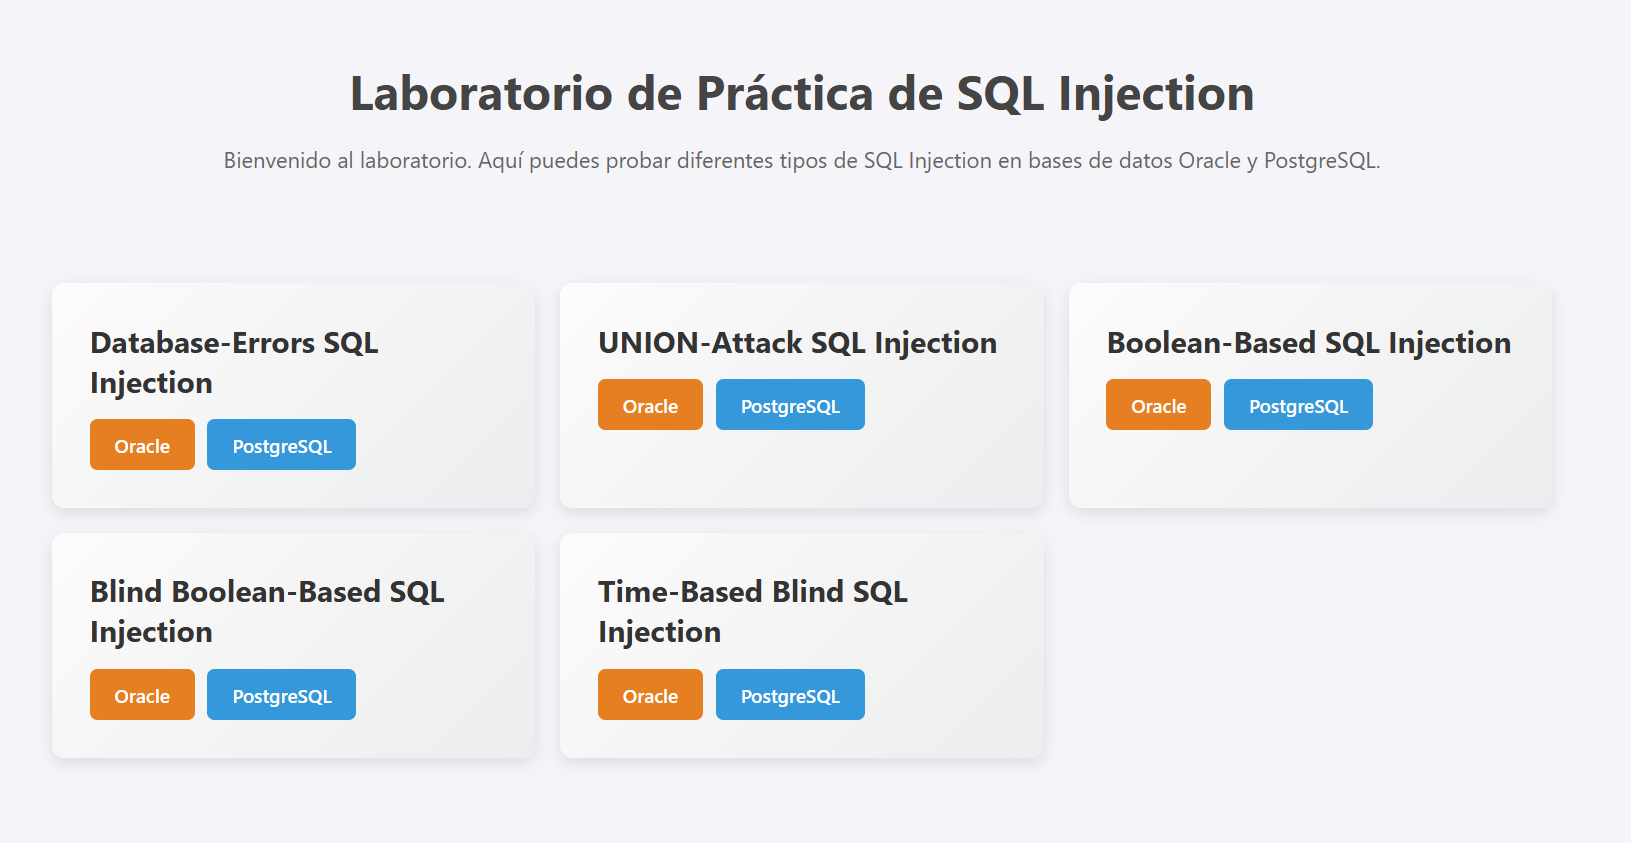
\includegraphics[width=0.8\textwidth]{Imagenes/MenuPrincipalLaboratorio.png}
    \caption{Página de inicio del laboratorio de inyecciones SQL}
\end{figure}

Para acceder a la sección especifica para esta inyección en el laboratorio, una vez desplegado el servidor, se debe seleccionar la opción \textit{Database-Errors SQL Injection}.

\begin{figure}[H]
    \centering
    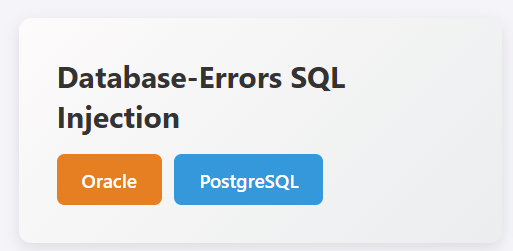
\includegraphics[width=0.8\textwidth]{Imagenes/error1.png}
    \caption{Opción de Database Errors en el laboratorio de inyecciones SQL}
\end{figure}

Como es posible observar, se tienen dos posibles opciones de trabajo de inyecciones en funcion de la base de datos que este trabajando de fondo, \textbf{Oracle} y \textbf{PostgreSQL}.
Como va a ser común entre las diferentes secciones en el laboratorio, se tiene un formulario básico de inicio de sesión con dos campos: \textit{usuario} y \textit{contraseña},
simulando lo que podria ser una ventana de login en una página web genérica.

\begin{figure}[H]
    \centering
    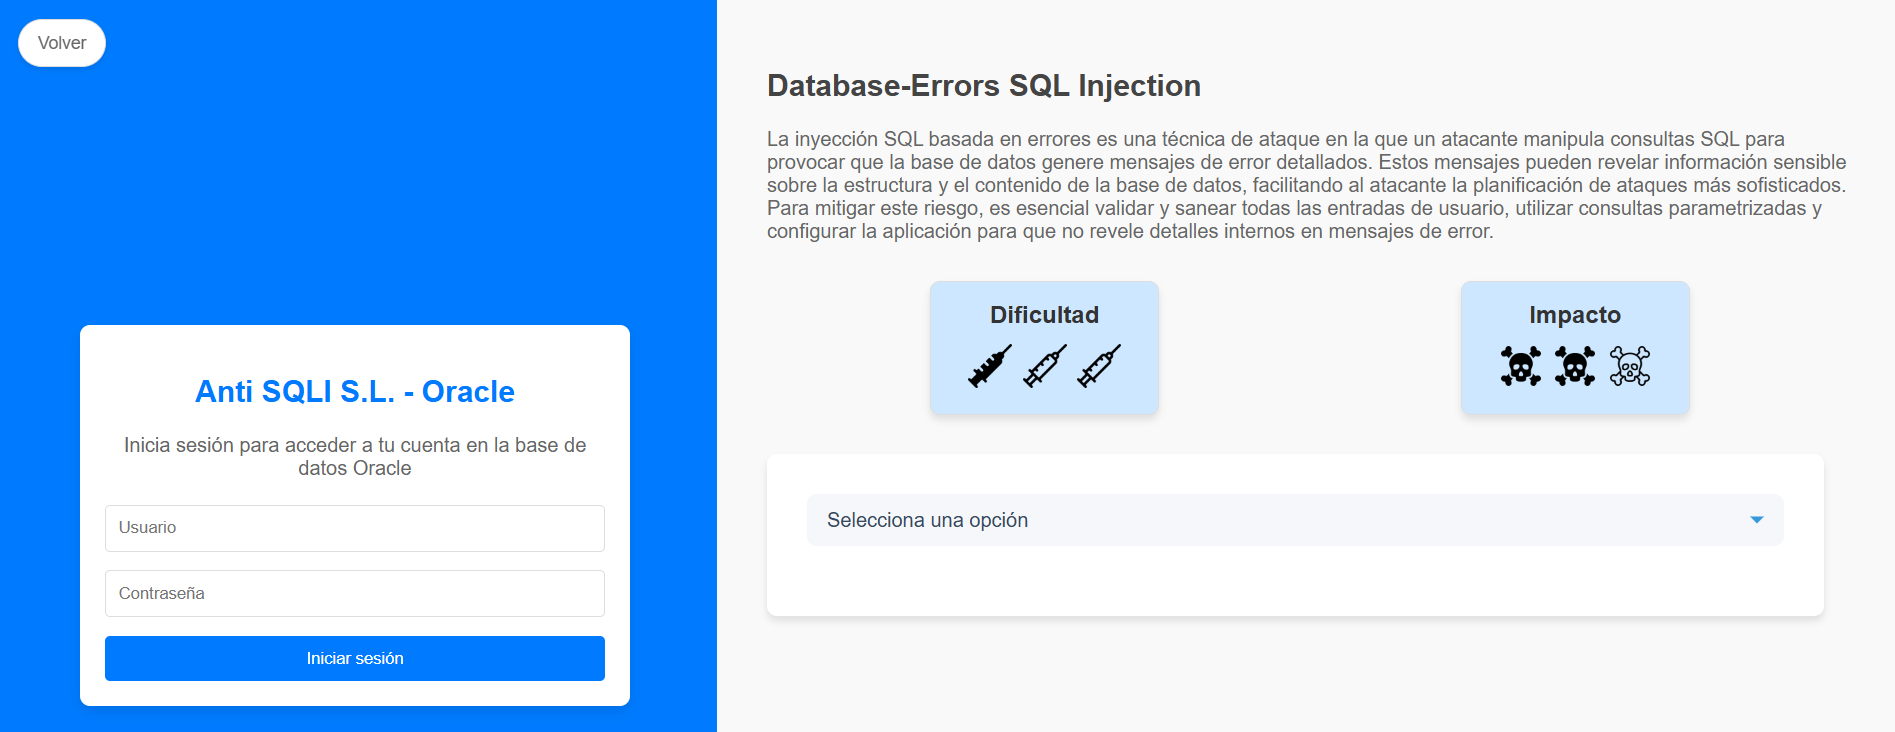
\includegraphics[width=0.8\textwidth]{Imagenes/error2.png}
    \caption{Formulario de inicio de sesión para inyección tipo Database-Errors}
\end{figure}

%Workflow de explotación (probando cada inyeccion). Mencionar al final que se ha documentado en oracle, 
%pero que en Postgre se sigue la misma logica de explotacion pero adaptando las inyecciones, y mostrar las inyecciones adaptadas, explicando las diferencias.

\subsection{Login sin credenciales válidas}
Como primer punto se ha decidido hacer mención al tipo de inyección para poder saltar el login sin credenciales válidas, ya que es un tipo de inyección fundamental y básica que va a funcionar en ambos SGBD
y en todas las subsecciones del laboratorio.

De modo que para realizar dicha inyección en el selector de inyecciones de la derecha, debajo de las tarjetas de información relevante se deberá seleccionar el tipo de inyección "Login sin credenciales válidas"
y muestra la siguiente información para introducir en los campos \textbf{Usuario} y \textbf{Contraseña}.

\begin{figure}[H]
    \centering
    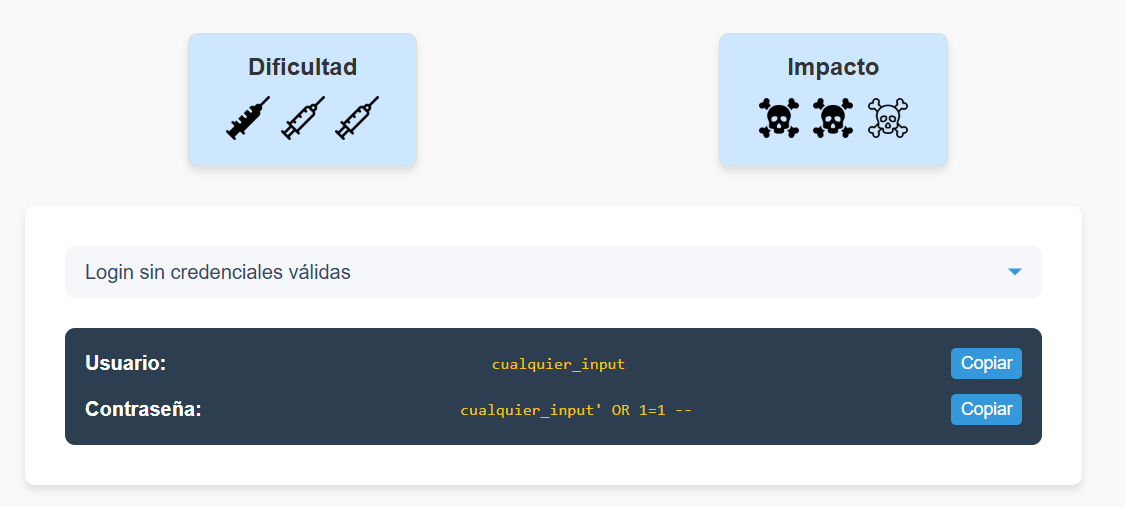
\includegraphics[width=0.8\textwidth]{Imagenes/error3.png}
    \caption{Datos a introducir en los campos del formulario}
\end{figure}

Como se puede observar en el código de inyección para el campo de la contraseña en el formulario, se aprovecha de la capacidad de SQL de poder trabajar con lógica booleana para inyectar
que la comprobación de que el conjunto \textit{usuario} y \textit{contraseña} esten en una tupla de la tabla o que 1 es igual a 1 (comentando lo que venga detras para evitar comporbaciones secundarias),
de modo que esta comprobación siempre va a ser cierta por la segunda parte de la comprobación.

\begin{lstlisting}[language=SQL]
SELECT * FROM Usuarios WHERE username = '(*@\textbf{cualquier\_input}@*)' AND password = '(*@\textbf{cualquier\_input' OR 1=1 --}@*)'
\end{lstlisting}

Atendiendo al diccionario de inyecciones en el código de la aplicación, en el caso de las inyecciones basadas en errores de la base de datos, se estaria usando la función con la vulnerabilidad
que permita mostrar este tipo inyección, denominada "login\_inseguro\_errors\_oracle".

Al ejecutar la función de inyección en el laboratorio, se obtiene un mensaje de éxito en la autenticación, lo que indica que la inyección ha sido exitosa 
y se ha logrado eludir la autenticación sin necesidad de credenciales válidas, puidendo observar la sentencia SQL total ejecutada y la tupla resultado obtenida de la tabla,
que debido a la naturaleza de la inyección, se ha devuelto la primera tupla de la tabla.

\begin{figure}[H]
    \centering
    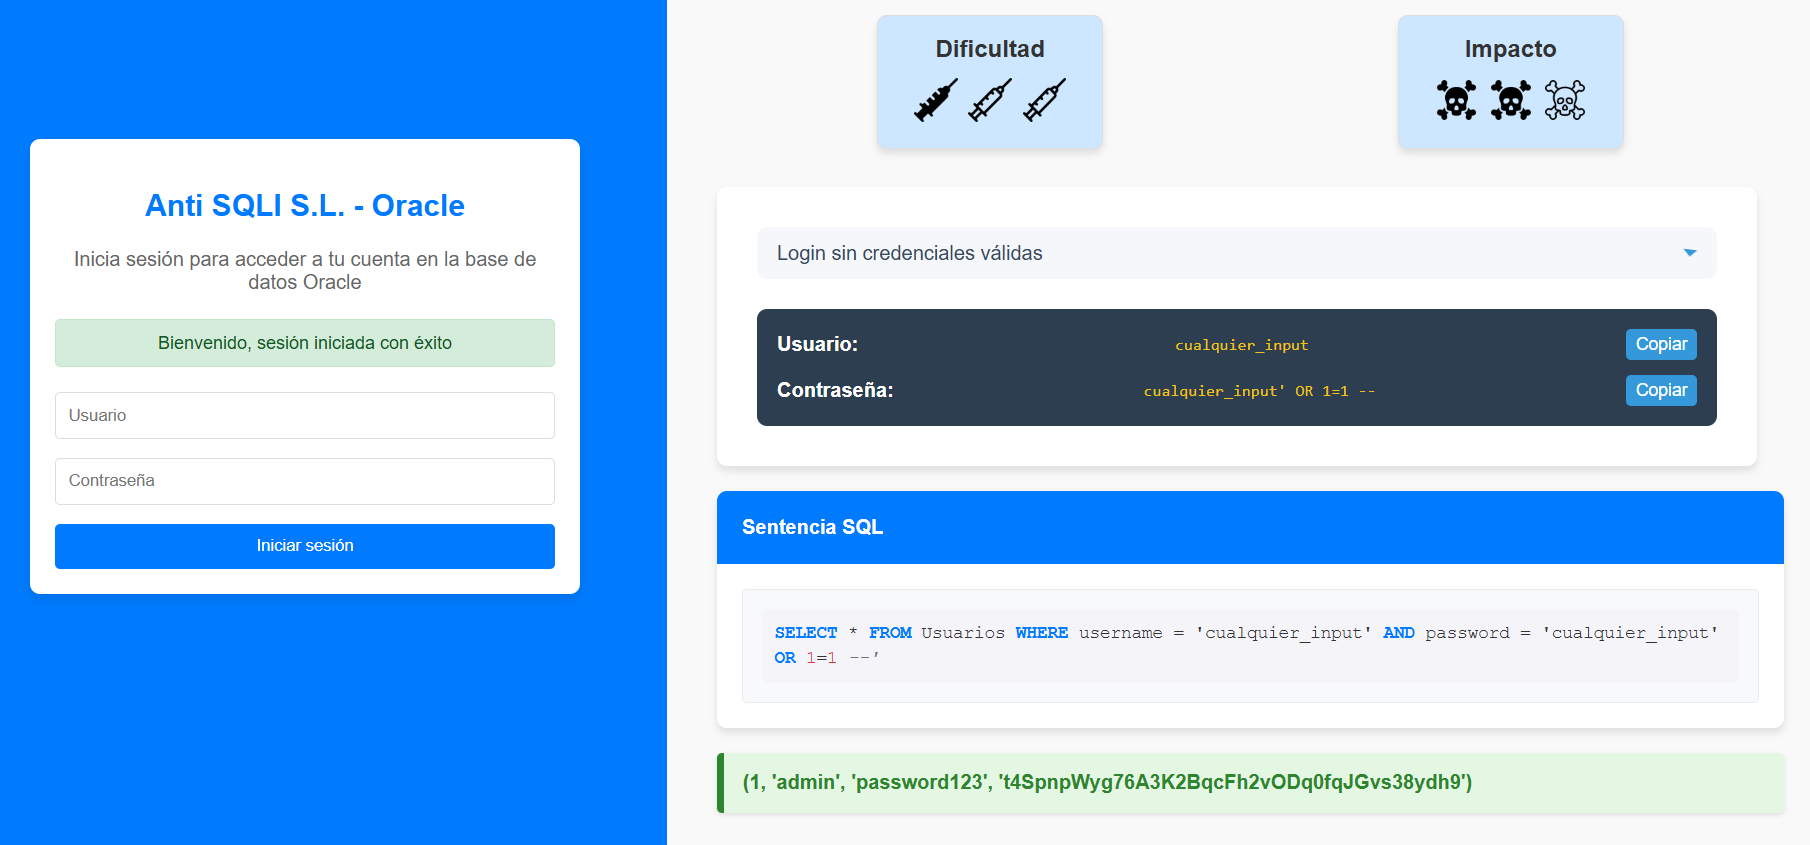
\includegraphics[width=0.8\textwidth]{Imagenes/error4.png}
    \caption{Resultado de la inyección para login sin credenciales válidas}
\end{figure}

\subsection{información sobre las tablas}

En la siguiente inyección se va a mostrar como se puede obtener información sobre las tablas de la base de datos, en este caso se va a obtener el nombre de las tablas de la base de datos.
Para realizar dicha inyección en el selector de inyecciones de la derecha, debajo de las tarjetas de información relevante se deberá seleccionar el tipo de inyección "Información sobre las tablas"
y muestra la siguiente información para introducir en los campos \textbf{Usuario} y \textbf{Contraseña}.

\subsection{Código vulnerable del login}

\begin{lstlisting}[language=Python]
    def login_inseguro_errors_oracle(username, password):
        print("---login---")
        print ("---login_inseguro_errors---")
        conexion = dbConectarOracle()  # Abre la conexión para autenticación
        if not conexion:
            print("Error: no se pudo conectar para autenticar.")
            return False
    
        sentencia = "SELECT * FROM Usuarios WHERE username = '"+username+"' AND password = '"+password+"'"
        try:
            cursor = conexion.cursor()
            cursor.execute(sentencia)
            usuario = cursor.fetchone()
    
            cursor.close()
            dbDesconectar(conexion)  # Cierra la conexión después de la autenticación
            if usuario:
                print("Usuario autenticado:", usuario)
                return {"resultado":usuario,"sentencia":sentencia, "auth":"true"}
            else:
                print("Usuario o contraseña incorrectos")
                return {"sentencia":sentencia}
        except PBD.DatabaseError as error:
            print("Error al autenticar usuario")
            print(error)
            dbDesconectar(conexion)
            return {"resultado":error, "sentencia":sentencia}
    \end{lstlisting}
    
La vulnerabilidad se encuentra en la concatenación de los valores de los campos \textit{usuario} y \textit{contraseña} en la consulta SQL, 
lo que permite al atacante manipular la lógica de la consulta para obtener acceso no autorizado al sistema; tal y como se ha visto anteriormente.

\section{Inyección basada en Union Attack}
La inyección SQL basada en \textbf{UNION} es una técnica en la que un atacante utiliza la cláusula UNION para combinar los resultados de una consulta legítima con datos maliciosamente solicitados, permitiendo extraer información sensible de la base de datos. 
Para llevar a cabo este ataque, el atacante identifica puntos vulnerables en la aplicación web, determina el \textbf{número de columnas} en la consulta original y luego inyecta una consulta maliciosa que utiliza \textbf{UNION SELECT} para unir los resultados deseados. 
Para prevenir este tipo de ataques, es esencial validar y sanear todas las entradas de usuario, utilizar consultas parametrizadas y aplicar el principio de privilegios mínimos en las cuentas de la base de datos.

\subsection{Mecanismo del ataque}

\begin{enumerate}
    \item \textbf{Identificación de puntos vulnerables:} El atacante busca parámetros de entrada en la aplicación web que interactúan directamente con la base de datos. Esto puede incluir campos de formularios, parámetros en la URL, cookies o encabezados HTTP.
    
    \item \textbf{Determinación del número de columnas:} Utilizando inyecciones como \texttt{ORDER BY} o consultas de prueba con \texttt{UNION SELECT NULL}, el atacante descubre el número de columnas en la consulta original. Esto asegura que la consulta maliciosa inyectada sea compatible con la estructura de la consulta legítima.
    
    \item \textbf{Construcción de la inyección:} Una vez identificados los parámetros vulnerables y el número de columnas, el atacante construye una consulta maliciosa utilizando \texttt{UNION SELECT}. Por ejemplo: \textit{http://example.com/page.php?id=1 UNION SELECT username, password FROM users}. En este caso, los datos sensibles de la tabla \texttt{users} son combinados con la consulta original.
\end{enumerate}

Para acceder a la sección especifica para esta inyección en el laboratorio, una vez desplegado el servidor, se debe seleccionar la opción \textit{UNION-Attack SQL Injection}.

\begin{figure}[H]
    \centering
    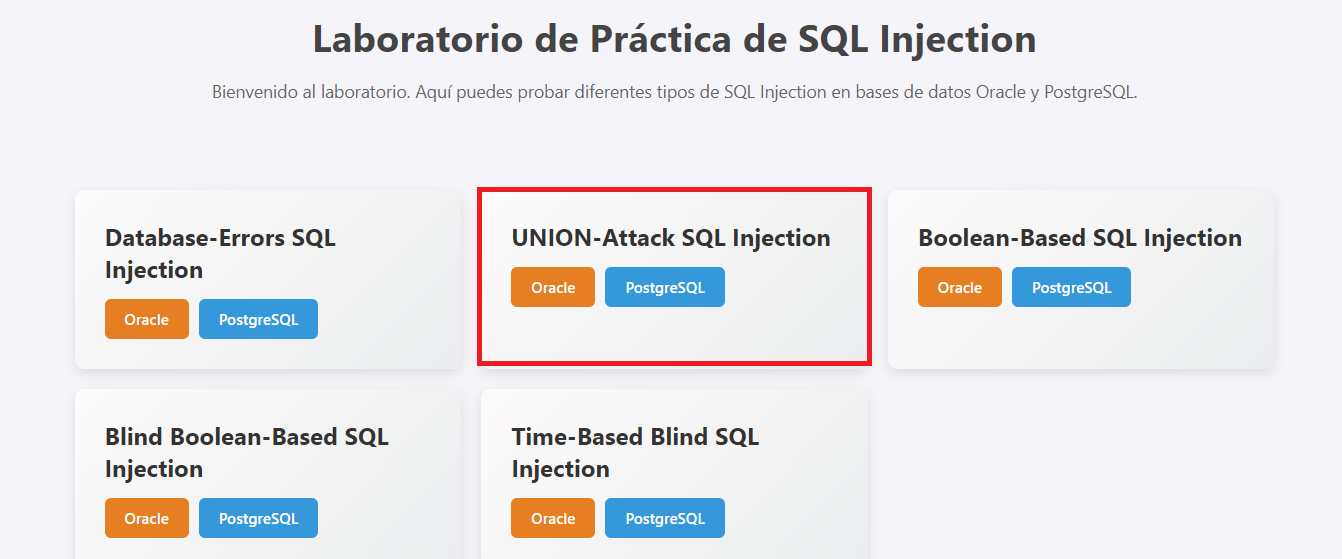
\includegraphics[width=0.8\textwidth]{Imagenes/union1.png}
    \caption{Opción de Union Attack en el laboratorio de inyecciones SQL}
\end{figure}

En esta sección, se tiene un formulario básico de inicio de sesión con dos campos: \textit{usuario} y \textit{contraseña}.

\begin{figure}[H]
    \centering
    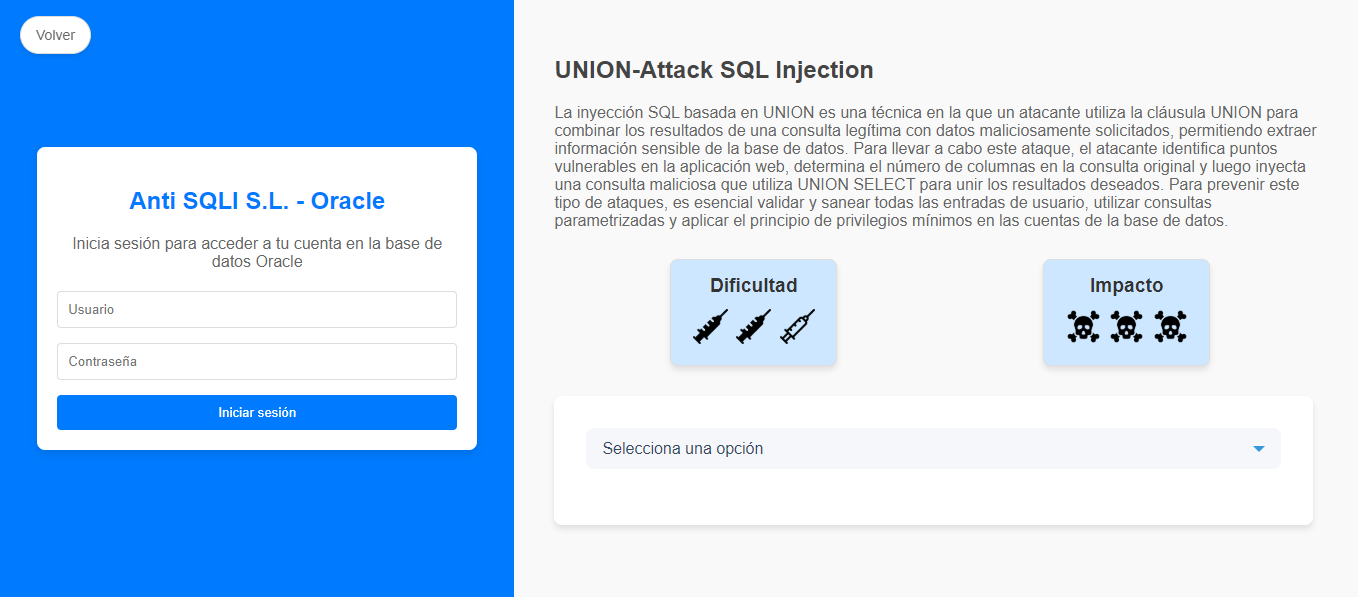
\includegraphics[width=0.8\textwidth]{Imagenes/union2.png}
    \caption{Formulario de inicio de sesión para Union Attack}
\end{figure}

%Workflow de explotación (probando cada inyeccion). Mencionar al final que se ha documentado en oracle, pero que en Postgre se sigue la misma logica de explotacion pero adaptando las inyecciones, y mostrar las inyecciones adaptadas, explicando las diferencias.
\subsection{Obtención de nombre de la base de datos}
En primer lugar, una de las cosas más básicas que se pueden obtener con este tipo de inyección SQL es el nombre de la base de datos con la que se está operando. Esta información, aunque pueda parecer trivial, resulta fundamental para los atacantes, ya que les permite personalizar sus ataques dependiendo del sistema de gestión de bases de datos que esté en uso.

En este laboratorio, para realizar este ataque en Oracle, se utiliza una inyección SQL que combina la consulta legítima con un \texttt{UNION SELECT}. En concreto, el payload malicioso es el siguiente:

\begin{lstlisting}[language=SQL]
cualquier_input' UNION SELECT 1, ora_database_name, NULL AS nombre_bd_relleno_1, NULL AS nombre_bd_relleno_2 FROM dual --
\end{lstlisting}

En este caso:
\begin{itemize}
    \item \texttt{ora\_database\_name}: Es una función específica de Oracle que devuelve el nombre de la base de datos activa.
    \item \texttt{NULL AS nombre\_bd\_relleno\_1} y \texttt{NULL AS nombre\_bd\_relleno\_2}: Se utilizan para completar el número de columnas requerido por la consulta original, ya que la cláusula \texttt{UNION SELECT} debe coincidir con el número y tipo de columnas de la consulta legítima.
    \item \texttt{dual}: Es una tabla especial de Oracle utilizada para ejecutar consultas que no necesitan datos de tablas reales.
\end{itemize}

\subsubsection{Explicación del funcionamiento}
La cláusula \texttt{UNION SELECT} combina los resultados de dos consultas SQL. En este caso, la inyección SQL modifica la consulta legítima original, añadiendo una nueva consulta que no está relacionada con los datos legítimos de la aplicación, pero que proporciona información sensible. Es importante tener en cuenta que la consulta maliciosa debe tener el mismo número de columnas que la consulta original.
Por ejemplo, si la consulta legítima tiene cuatro columnas (en este caso en la tabla \textit{usuarios} existen las columnas \texttt{id}, \texttt{username}, \texttt{password} y \texttt{session\_cookie}), la inyección debe proporcionar exactamente cuatro valores en su cláusula \texttt{UNION SELECT}. De lo contrario, Oracle devolverá un error debido a la incompatibilidad de columnas. Para esta inyección, solo interesa el valor de \texttt{ora\_database\_name}, pero se incluyen \texttt{1} y \texttt{NULL} como valores de relleno para las demás columnas requeridas.

Al ejecutar esta inyección, el atacante obtiene el nombre de la base de datos en el campo correspondiente, que se muestra en la interfaz del laboratorio como un valor destacado en la salida del ataque.

\begin{figure}[H]
    \centering
    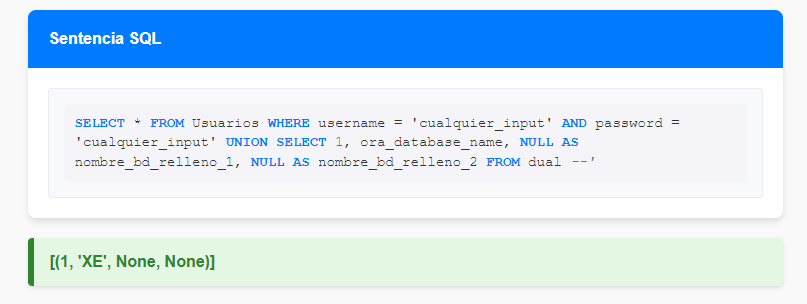
\includegraphics[width=0.8\textwidth]{Imagenes/union3.png}
    \caption{Obtención del nombre de la base de datos en Oracle}
\end{figure}

\subsection{Obtención de la versión de la base de datos}
Otro de los datos fundamentales que se pueden obtener mediante una inyección SQL basada en \texttt{UNION SELECT} es la versión de la base de datos en uso. Este dato proporciona información valiosa al atacante, ya que permite identificar la versión exacta del sistema de gestión de bases de datos (SGBD) Oracle. Con esta información, es posible adaptar los ataques a las vulnerabilidades específicas de esa versión.

En este laboratorio, se utiliza la siguiente inyección SQL para obtener la versión de la base de datos Oracle:

\begin{lstlisting}[language=SQL]
cualquier_input' UNION SELECT NULL, banner, NULL, NULL FROM v$version WHERE banner LIKE 'Oracle%' --
\end{lstlisting}

En este caso:
\begin{itemize}
    \item \texttt{banner}: Es una columna de la vista \texttt{v\$version}, que contiene información detallada sobre la versión y el entorno de la base de datos. Esta columna proporciona información como la edición de la base de datos, la versión y el sistema operativo sobre el que está ejecutándose.
    \item \texttt{v\$version}: Es una vista de diccionario del sistema en Oracle que almacena información sobre las versiones de los componentes del sistema de gestión de bases de datos. Esta vista es ampliamente utilizada tanto en administración legítima como en ataques para identificar detalles del entorno.
    \item \texttt{NULL}: Al igual que en otras inyecciones \texttt{UNION SELECT}, los valores \texttt{NULL} se utilizan para rellenar las columnas restantes en la consulta inyectada. Esto garantiza que la consulta inyectada tenga el mismo número de columnas que la consulta legítima original, evitando errores de sintaxis en la ejecución.
    \item \texttt{WHERE banner LIKE 'Oracle\%'}: Este filtro se aplica para restringir los resultados de la consulta únicamente a las filas que contienen información relevante sobre la base de datos Oracle. La condición \texttt{LIKE 'Oracle\%'} asegura que solo se devuelvan banners relacionados con la base de datos Oracle, excluyendo otros componentes potenciales del sistema.
\end{itemize}

\subsubsection{Explicación del funcionamiento}
El objetivo de esta inyección es aprovechar la estructura de la vista \texttt{v\$version} para obtener la versión exacta de la base de datos. La consulta inyectada utiliza \texttt{UNION SELECT} para combinar los resultados de la consulta legítima con una consulta que devuelve el contenido de la columna \texttt{banner} de la vista \texttt{v\$version}. Al ejecutar esta inyección, el valor de la versión se presenta en el campo correspondiente de la interfaz de la aplicación, proporcionando al atacante la información necesaria para ajustar ataques posteriores.

Al ejecutar esta inyección, el atacante obtiene la versión de la base de datos en el campo correspondiente, que se muestra en la interfaz del laboratorio como un valor destacado en la salida del ataque.

\begin{figure}[H]
    \centering
    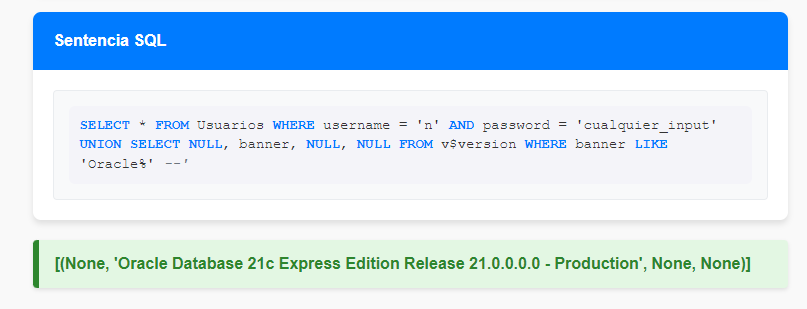
\includegraphics[width=0.8\textwidth]{Imagenes/union4.png}
    \caption{Obtención de la versión de la base de datos en Oracle}
\end{figure}

\subsection{Obtención de todas las tablas de la base de datos}
Un paso clave en un ataque avanzado es obtener un listado de todas las tablas de la base de datos. Este tipo de información permite a un atacante identificar las estructuras de datos disponibles, lo que facilita la selección de objetivos específicos, como tablas que almacenan credenciales, datos confidenciales o información sensible. Para lograr esto, se puede realizar una inyección SQL que extraiga información directamente de las vistas del sistema disponibles en la base de datos.

En este laboratorio, se utiliza la siguiente inyección SQL para obtener un listado de las tablas de la base de datos Oracle bajo el esquema del propietario \texttt{SYSTEM}:

\begin{lstlisting}[language=SQL]
cualquier_input' UNION SELECT 1, NULL, OWNER, TABLE_NAME FROM all_tables WHERE OWNER='SYSTEM' -- AND password = 'cualquier_input'
\end{lstlisting}

En este caso:
\begin{itemize}
    \item \texttt{OWNER}: Es una columna de la vista \texttt{ALL\_TABLES} que contiene el nombre del propietario (esquema) al que pertenece cada tabla en la base de datos. En este caso, se está filtrando específicamente al propietario \texttt{SYSTEM}, que normalmente contiene tablas relacionadas con la administración de la base de datos.
    \item \texttt{TABLE\_NAME}: Es otra columna de la vista \texttt{ALL\_TABLES} que contiene el nombre de cada tabla dentro del esquema indicado. Esta es la información objetivo del ataque, ya que revela todos los nombres de las tablas disponibles.
    \item \texttt{NULL}: Se utiliza como valor de relleno para columnas que no son relevantes en la consulta inyectada. Esto asegura que el número de columnas en la consulta inyectada coincida con el de la consulta legítima, evitando errores de ejecución.
    \item \texttt{ALL\_TABLES}: Es una vista del diccionario de datos de Oracle que muestra todas las tablas accesibles al usuario actual, incluidas las de otros esquemas a las que tenga permisos.
    \item \texttt{WHERE OWNER='SYSTEM'}: Este filtro se aplica para limitar los resultados de la consulta a las tablas que pertenecen al esquema \texttt{SYSTEM}. Esto permite enfocar el ataque en un área específica de la base de datos.
    \item \texttt{-- AND password = 'cualquier\_input'}: El uso del comentario (\texttt{--}) elimina cualquier condición adicional en la consulta original, como la verificación de contraseñas, asegurando que la consulta inyectada se ejecute sin restricciones. En este caso la inyección se realiza en el campo \textbf{}
\end{itemize}

\subsubsection{Explicación del funcionamiento}
La consulta inyectada aprovecha la vista \texttt{ALL\_TABLES} para obtener un listado de todas las tablas accesibles en el esquema \texttt{SYSTEM}. La combinación de \texttt{UNION SELECT} con esta vista permite extraer datos estructurados directamente del diccionario de datos de Oracle.

La estructura de la consulta original se mantiene al incluir cuatro valores en la inyección (\texttt{1}, \texttt{NULL}, \texttt{OWNER} y \texttt{TABLE\_NAME}), lo que coincide con el número de columnas de la consulta legítima. Esto evita errores de sintaxis y asegura que los resultados de la inyección se combinen correctamente con los de la consulta original.

Al ejecutar esta inyección, el atacante obtiene todos los nombres de las tablas almacenadas en la base de datos.

\begin{figure}[H]
    \centering
    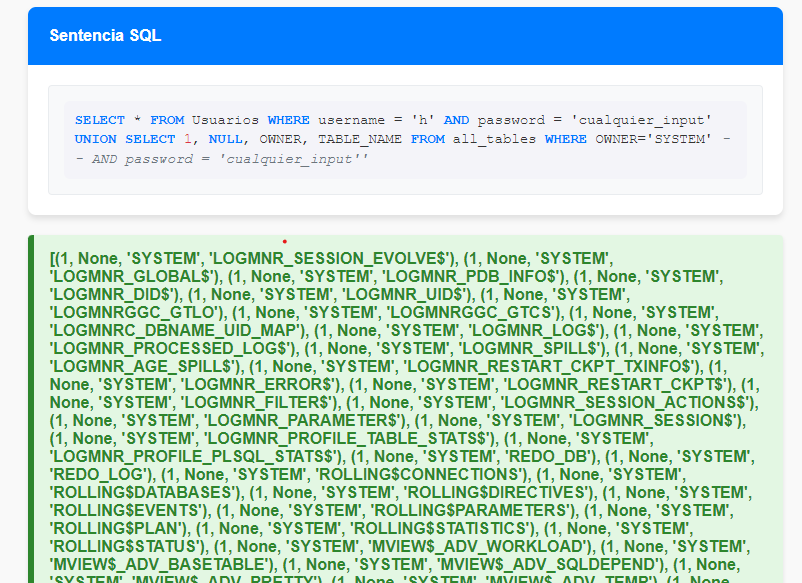
\includegraphics[width=0.8\textwidth]{Imagenes/union5.png}
    \caption{Obtención de tablas de la base de datos en Oracle}
\end{figure}

Al ejecutar una inyección SQL que consulta la vista \texttt{ALL\_TABLES}, es común que el resultado incluya tablas creadas por defecto por Oracle, como aquellas asociadas al sistema o utilizadas internamente para la administración de la base de datos. Para centrarse únicamente en tablas relevantes para el atacante, se pueden aplicar filtros adicionales en la cláusula \texttt{WHERE} de la inyección.

Un ejemplo de una inyección con estos filtros aplicados es el siguiente:

\begin{lstlisting}[language=SQL]
cualquier_input' UNION SELECT 1, NULL, OWNER, TABLE_NAME FROM all_tables 
WHERE OWNER = 'SYSTEM' 
AND TABLE_NAME NOT LIKE '%$%' 
AND TABLE_NAME NOT LIKE 'SYS%' 
AND TABLE_NAME NOT LIKE 'LOGMNR%' --
\end{lstlisting}

En este caso:
\begin{itemize}
    \item \texttt{TABLE\_NAME NOT LIKE '\%\$\%'}: Filtra tablas cuyos nombres contienen el carácter \texttt{\$}, que generalmente son tablas de sistema utilizadas internamente por Oracle para la gestión de metadatos o componentes específicos.
    \item \texttt{TABLE\_NAME NOT LIKE 'SYS\%'}: Excluye tablas cuyos nombres comienzan con \texttt{SYS}, ya que estas suelen pertenecer al esquema del sistema (\texttt{SYS}) y no son de interés para la mayoría de los ataques.
    \item \texttt{TABLE\_NAME NOT LIKE 'LOGMNR\%'}: Elimina tablas relacionadas con la funcionalidad de \texttt{LogMiner} de Oracle, una herramienta utilizada para analizar registros de transacciones y que, en la mayoría de los casos, no contiene datos directamente útiles para los atacantes.
\end{itemize}

Al aplicar estos filtros, los resultados de la consulta se limitan a las tablas más relevantes, lo que facilita el análisis y reduce el ruido en el proceso de reconocimiento. Esto es especialmente útil en entornos con un gran número de tablas, donde los resultados pueden ser abrumadores si se incluyen todas las tablas creadas por defecto por Oracle.

Por ejemplo, al filtrar las tablas de sistema, el atacante puede enfocarse en tablas creadas por el administrador o los desarrolladores de la base de datos, que probablemente contengan información sensible o relacionada con las funcionalidades de la aplicación.

El laboratorio refleja esta estrategia de filtrado mostrando únicamente las tablas relevantes después de ejecutar la inyección filtrada. Esto permite a los participantes observar cómo una consulta más específica puede ser más efectiva en un ataque real.

\begin{figure}[H]
    \centering
    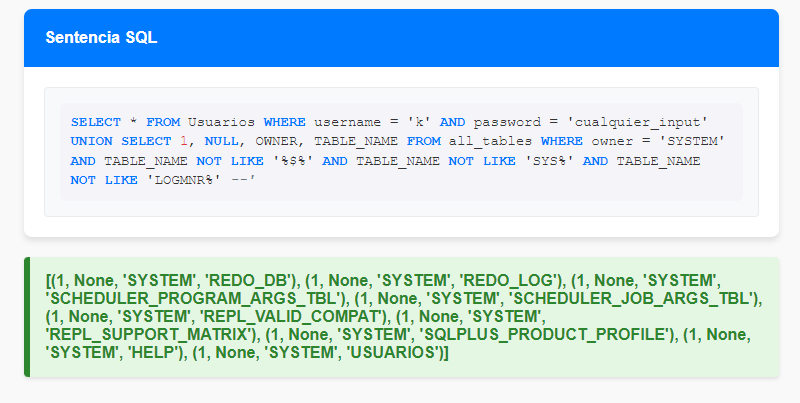
\includegraphics[width=0.8\textwidth]{Imagenes/union6.png}
    \caption{Obtención de tablas filtradas en Oracle}
\end{figure}


%Mostrar y documentar código de login vulnerable (si no se ha documentado ya en una inyeccion previa)



%------------------------------------------------------------------------------------------------------

%Conclusiones (mostrar código de login seguro)
%Anexo (Cajon desastre para codigo completo, ejecuciones completas, etc)
%Bibliografia (PortSwigger, OWASP, etc)

\end{document}
